\documentclass{subfiles}

\begin{document}

  \chapter*{Apéndice A: Manual de uso}
  \label{sec:anexo_manual_de_uso}
  \addcontentsline{toc}{chapter}{\protect\numberline{}A. Manual de uso}

        El caso de uso principal del usuario será, generalmente, el siguiente:

\begin{figure}[H]
\centering
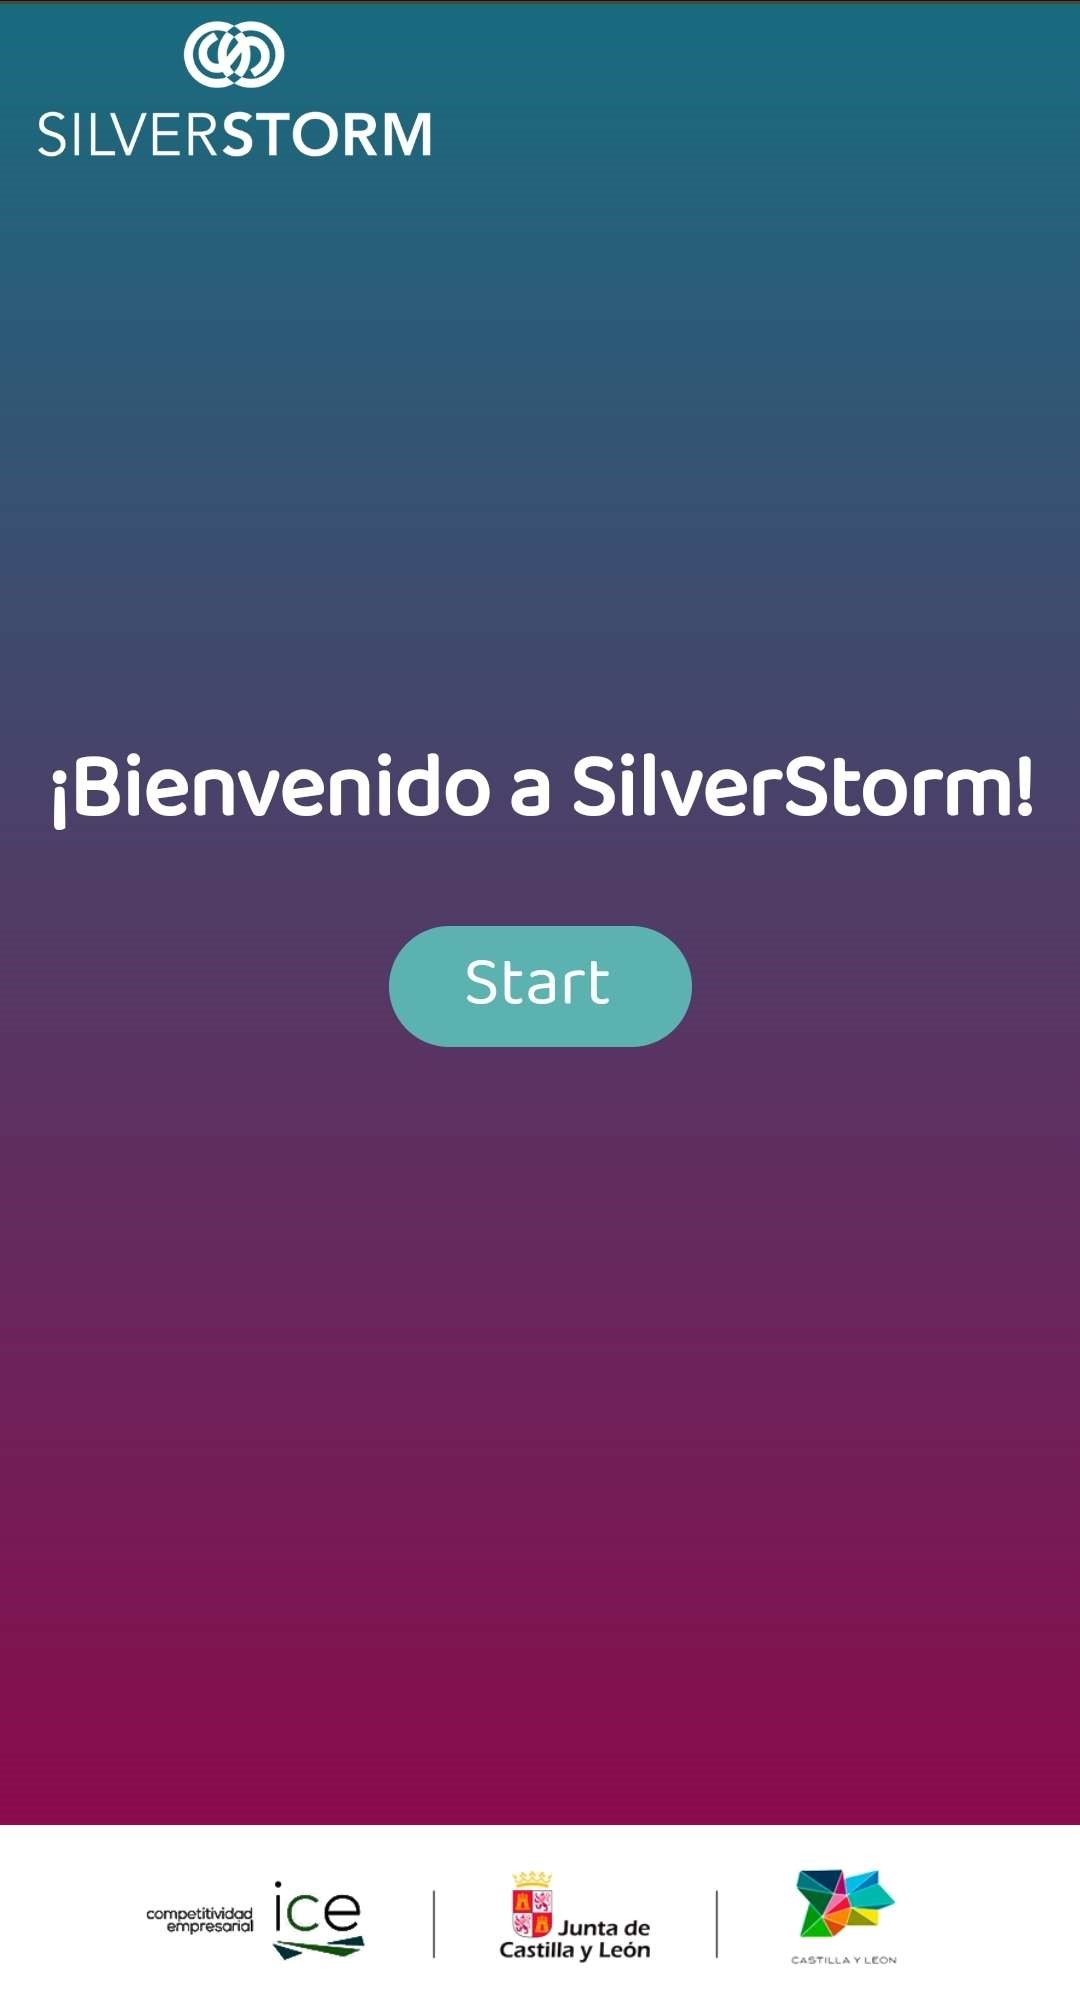
\includegraphics[width=0.25\textwidth]{1_landing_page.jpg}
\caption{El usuario accede a la landing page.}
\label{fig:1_landing_page}
\end{figure}

        \paragraph{}
        Nada más entrar en la aplicación, como se explicó anteriormente, el usuario podrá ver la \textit{landing page}, una página estática sencilla donde aparecerá un botón que servirá para cargar los modelos necesarios y lanzar la sesión de \ra (figura \ref{fig:1_landing_page}). 

\begin{figure}[H]
\centering
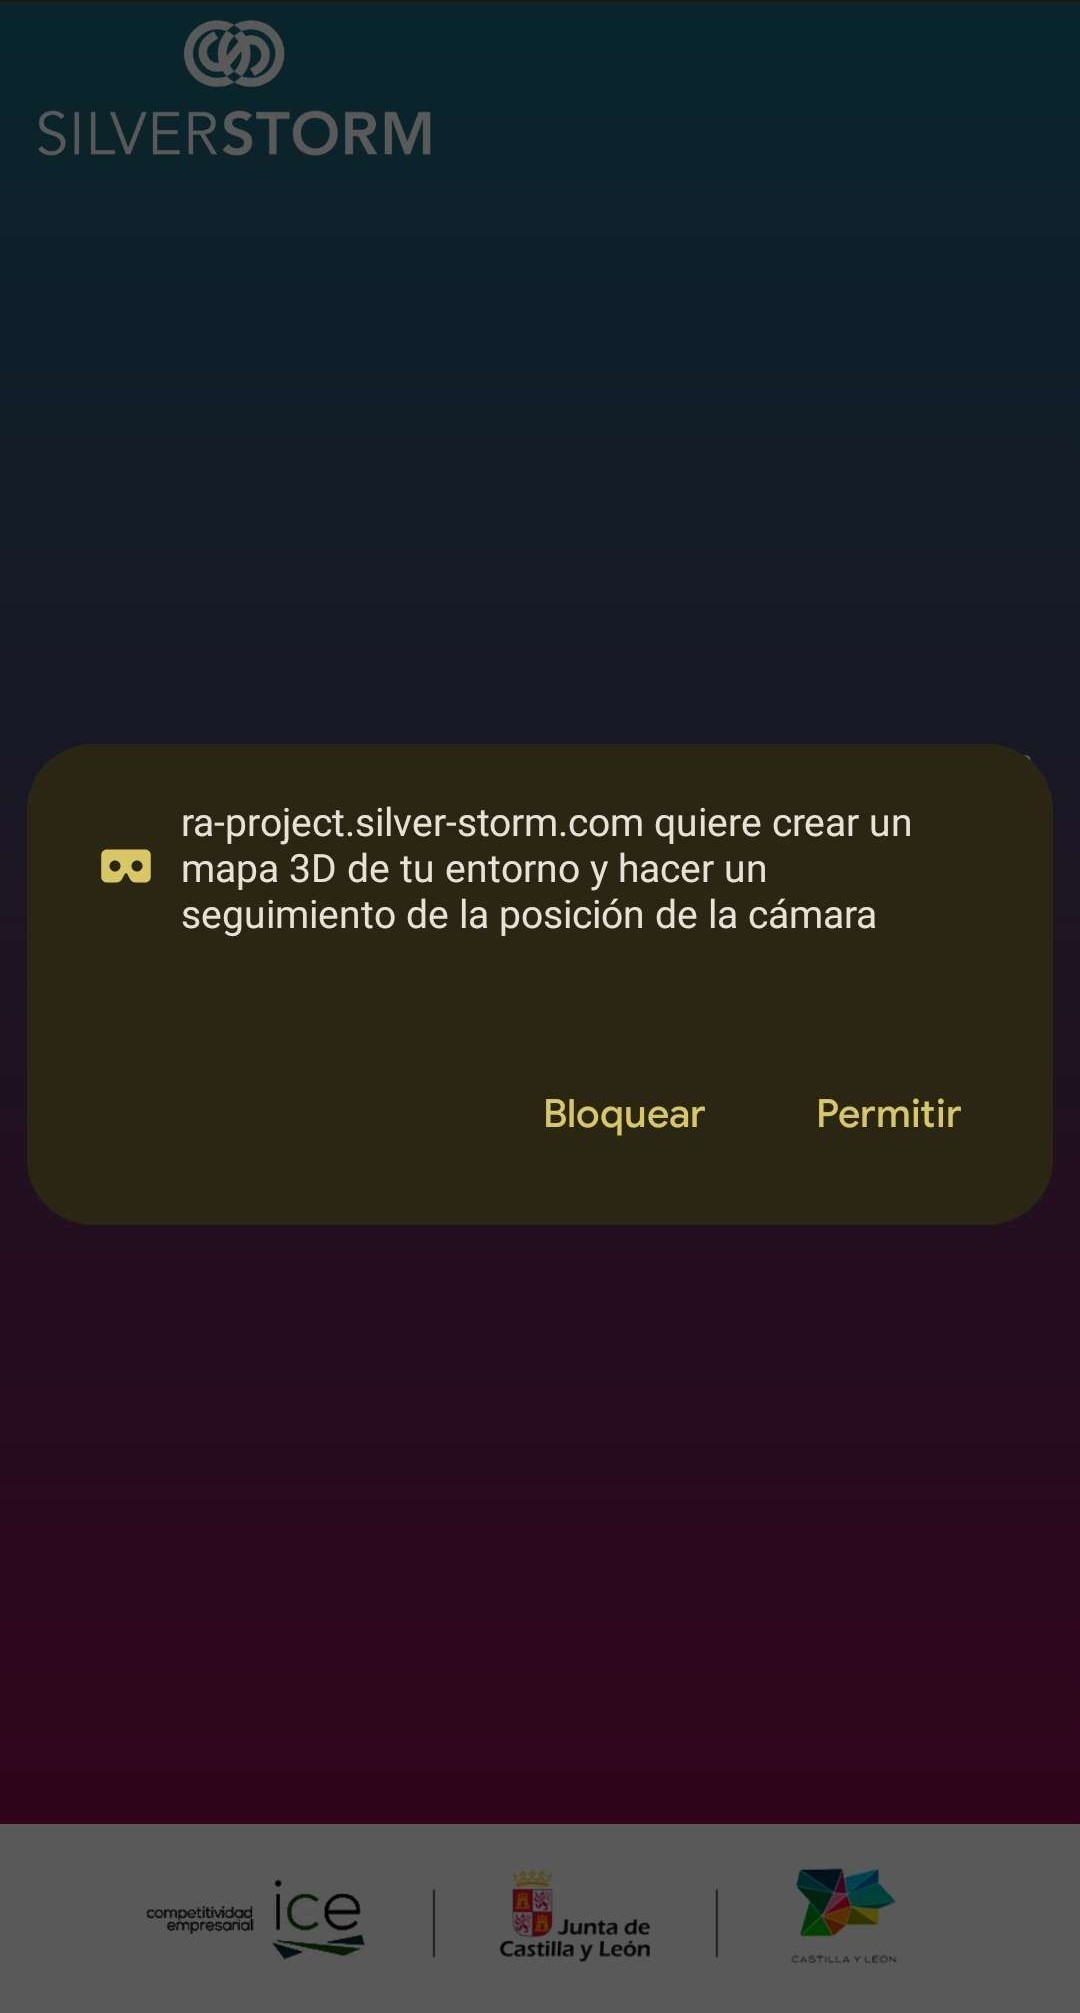
\includegraphics[width=0.25\textwidth]{2_permissions.jpg}
\caption{Se solicitan permisos al usuario.}
\label{fig:2_permissions}
\end{figure}

        \paragraph{}
        Al pulsar sobre el botón, el navegador avisará al usuario de que se pretenden utilizar funciones asociadas a la \ra (figura \ref{fig:2_permissions}). En concreto, el mensaje avisa al usuario sobre la posibilidad de crear mapas 3D del entorno y el seguimiento de la posición de la cámara. Si el usuario ha dado estos permisos previamente, el sistema no lo volverá a preguntar.

\begin{figure}[H]
\centering
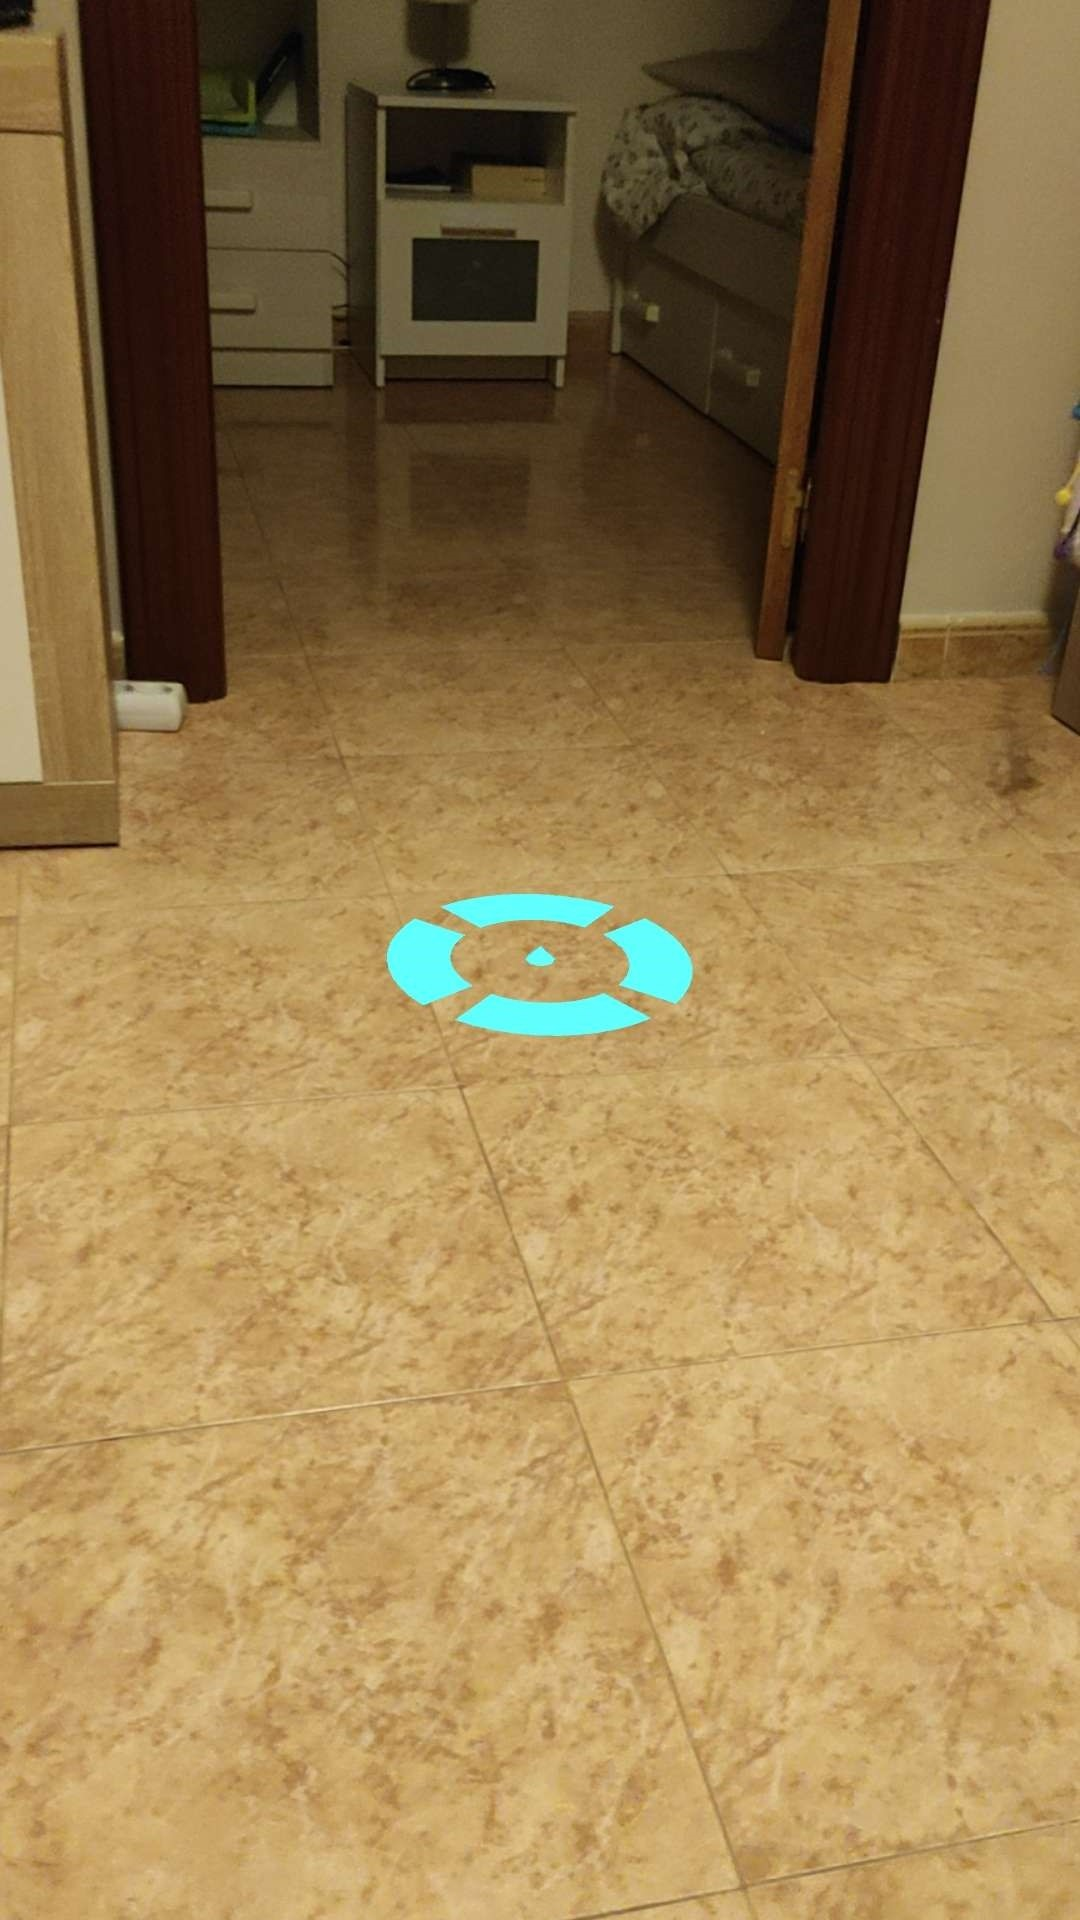
\includegraphics[width=0.2\textwidth]{3_reticle.jpg}
\caption{La aplicación muestra las imágenes de la cámara y coloca la retícula sobre la superficie detectada.}
\label{fig:3_reticle}
\end{figure}

        \paragraph{}
        Una vez el usuario conceda los permisos, la aplicación accederá a la cámara, donde utilizará las imágenes recibidas para calcular superficies (figura \ref{fig:3_reticle}). Una vez detecte una superficie horizontal, el sistema mostrará la retícula. Es posible que el usuario necesite mover suavemente el dispositivo durante varios segundos apuntando hacia el suelo.

\begin{figure}[H]
\centering
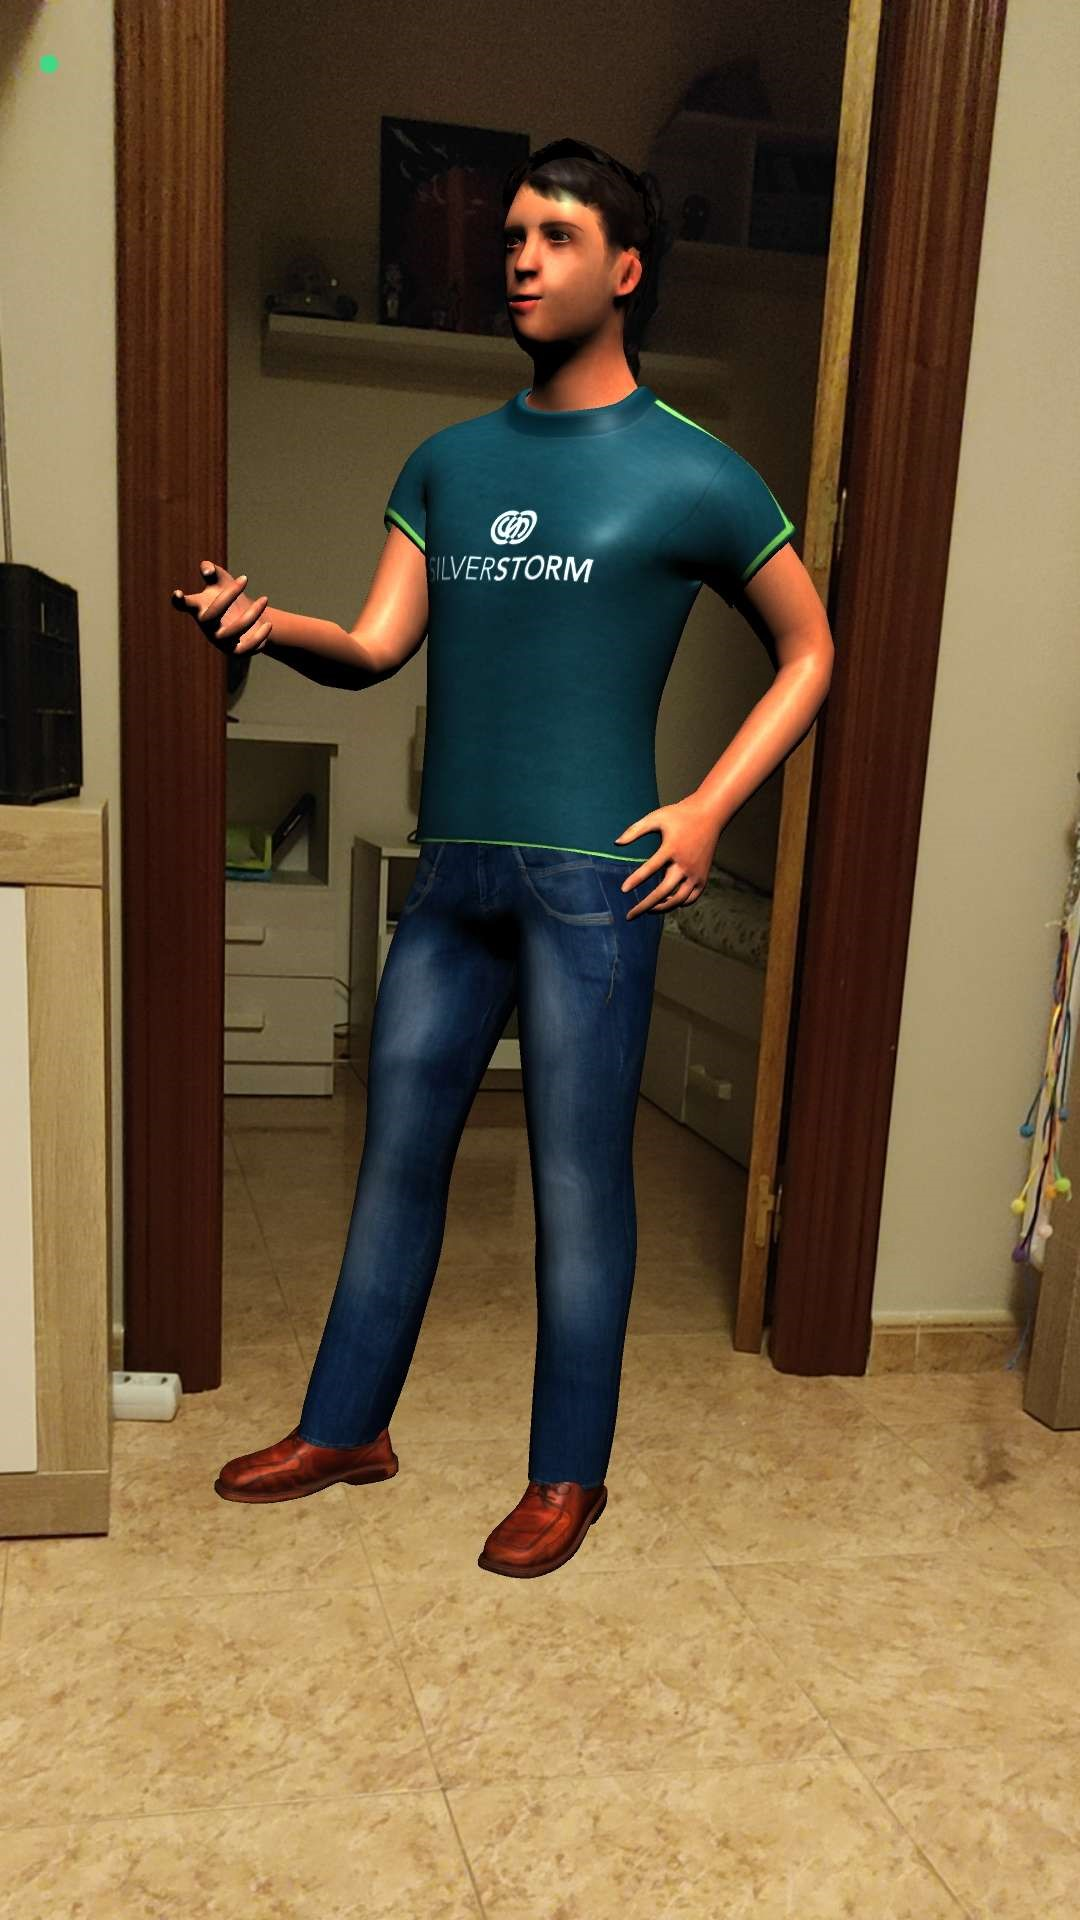
\includegraphics[width=0.2\textwidth]{4_model_appears.jpg}
\caption{Al pulsar sobre la pantalla, aparece el modelo y comienza su <<discurso>>.}
\label{fig:4_model_appears}
\end{figure}

        \paragraph{}
        Una vez se muestre la retícula, y no antes, el usuario podrá mostrar al modelo en 3D al pulsar sobre la pantalla, apareciendo allá donde estuviese la retícula (figura \ref{fig:4_model_appears}). Además, el modelo comenzará a hablar y moverse y la retícula desaparecerá al realizar esta acción. Su voz aumentará o disminuirá en relación a la distancia entre la cámara y el modelo, y el sonido se percibirá por los auriculares en relación a la posición del modelo con respecto a la cámara.

\begin{figure}[H]
\centering
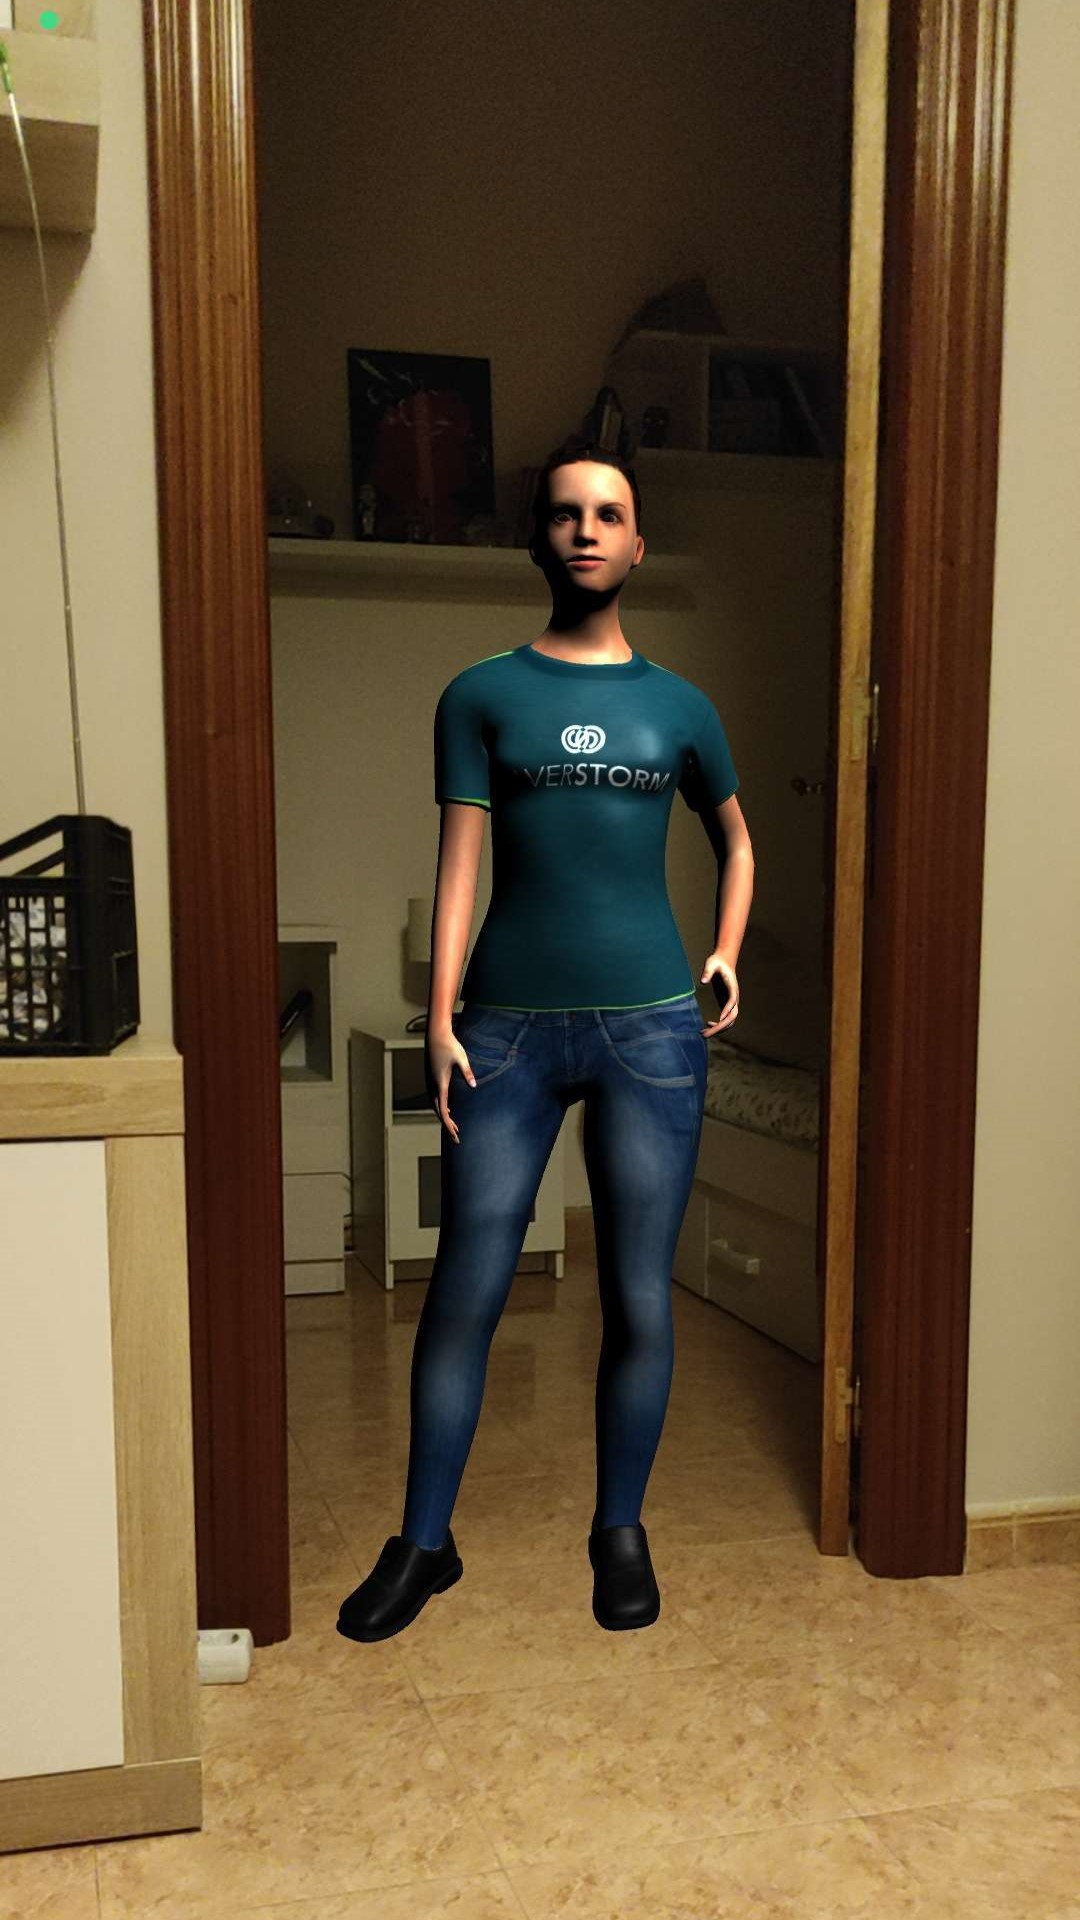
\includegraphics[width=0.2\textwidth]{5_alternate_model.jpg}
\caption{La selección del modelo es completamente aleatoria.}
\label{fig:5_alternate_model}
\end{figure}

        \paragraph{}
        El modelo utilizado se seleccionará de manera completamente aleatoria, pudiendo aparecer uno de dos diseños distintos (figura \ref{fig:5_alternate_model}). Cada uno tendrá su propia voz, aunque las animaciones son similares.

\begin{figure}[H]
\centering
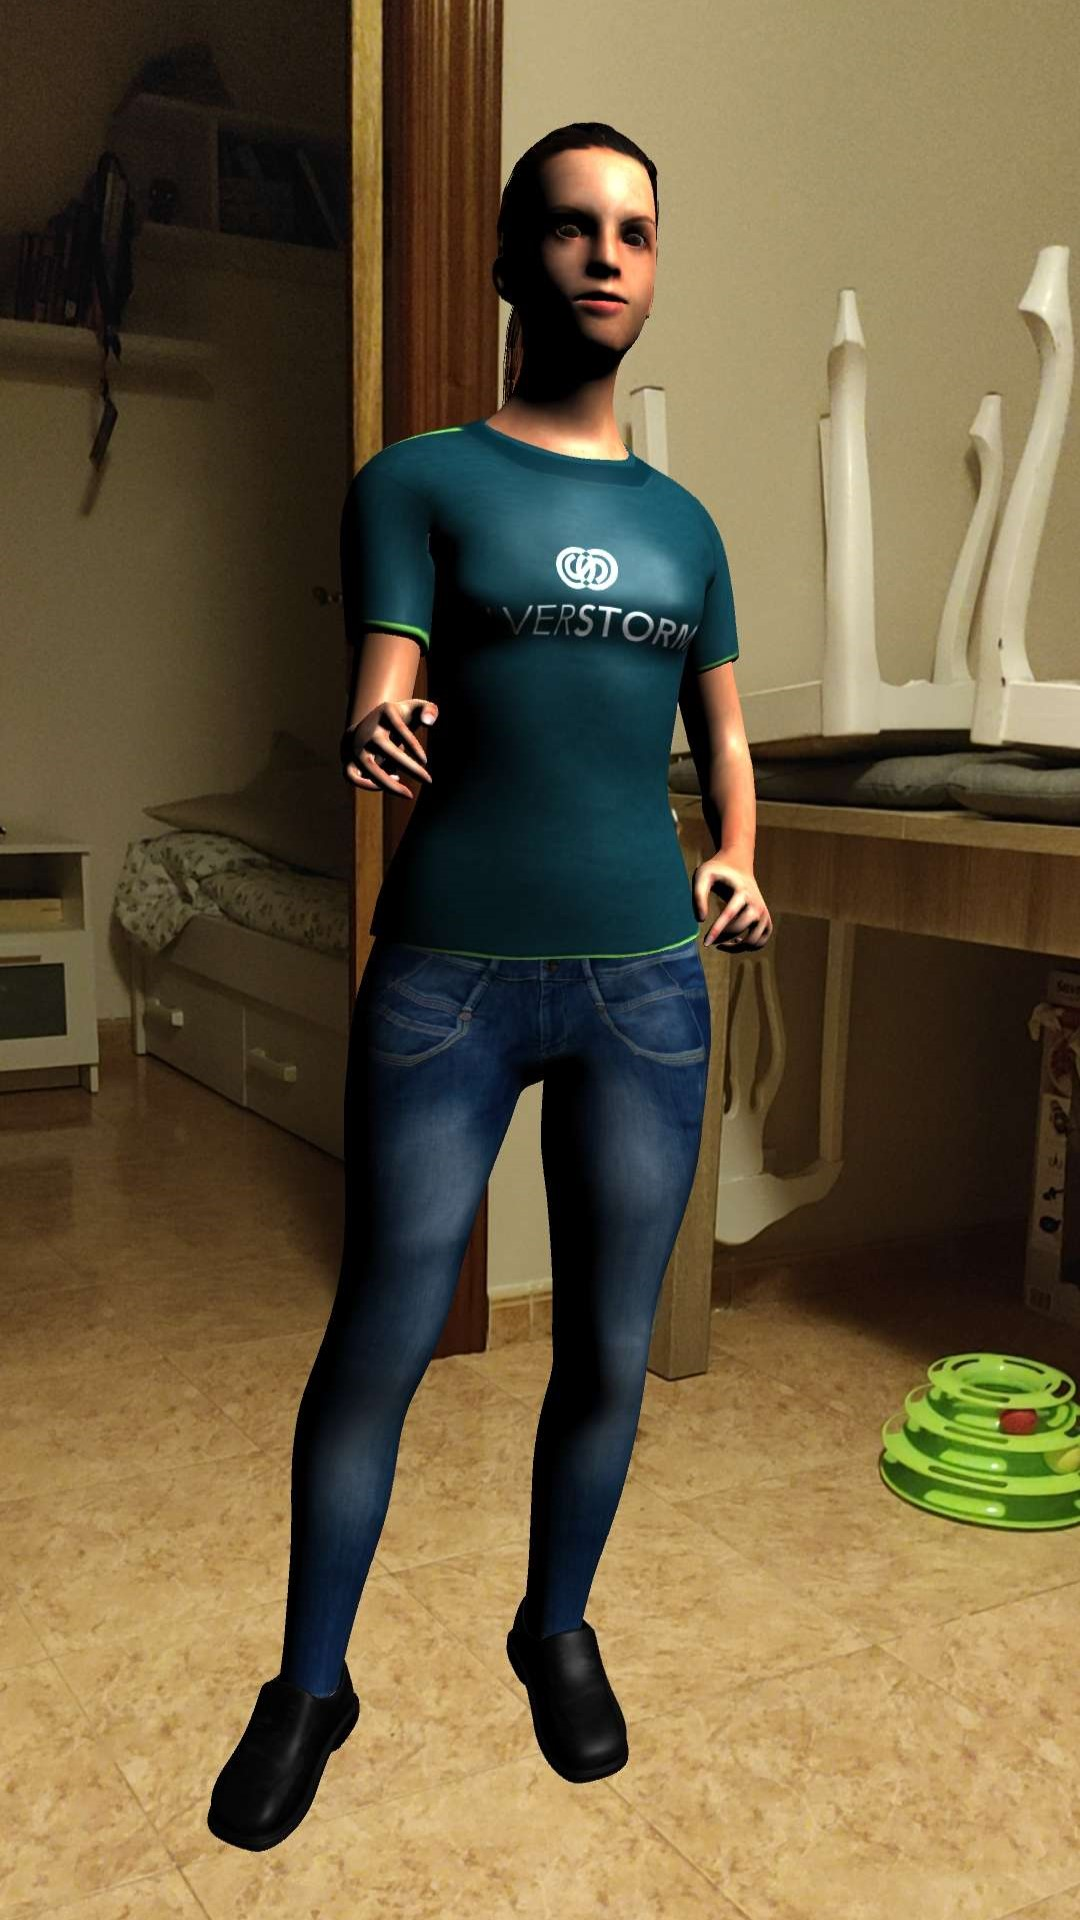
\includegraphics[width=0.2\textwidth]{6_moving_model.jpg}
\caption{El modelo podrá ser desplazado de lugar.}
\label{fig:6_moving_model}
\end{figure}

        \paragraph{}
        Una vez cargado el modelo y mostrado en la sesión, el usuario podrá volver a pulsar sobre la pantalla para mover al modelo, sin que esto interrumpa la animación o la voz del modelo (figura \ref{fig:6_moving_model}.

\begin{figure}[H]
\centering
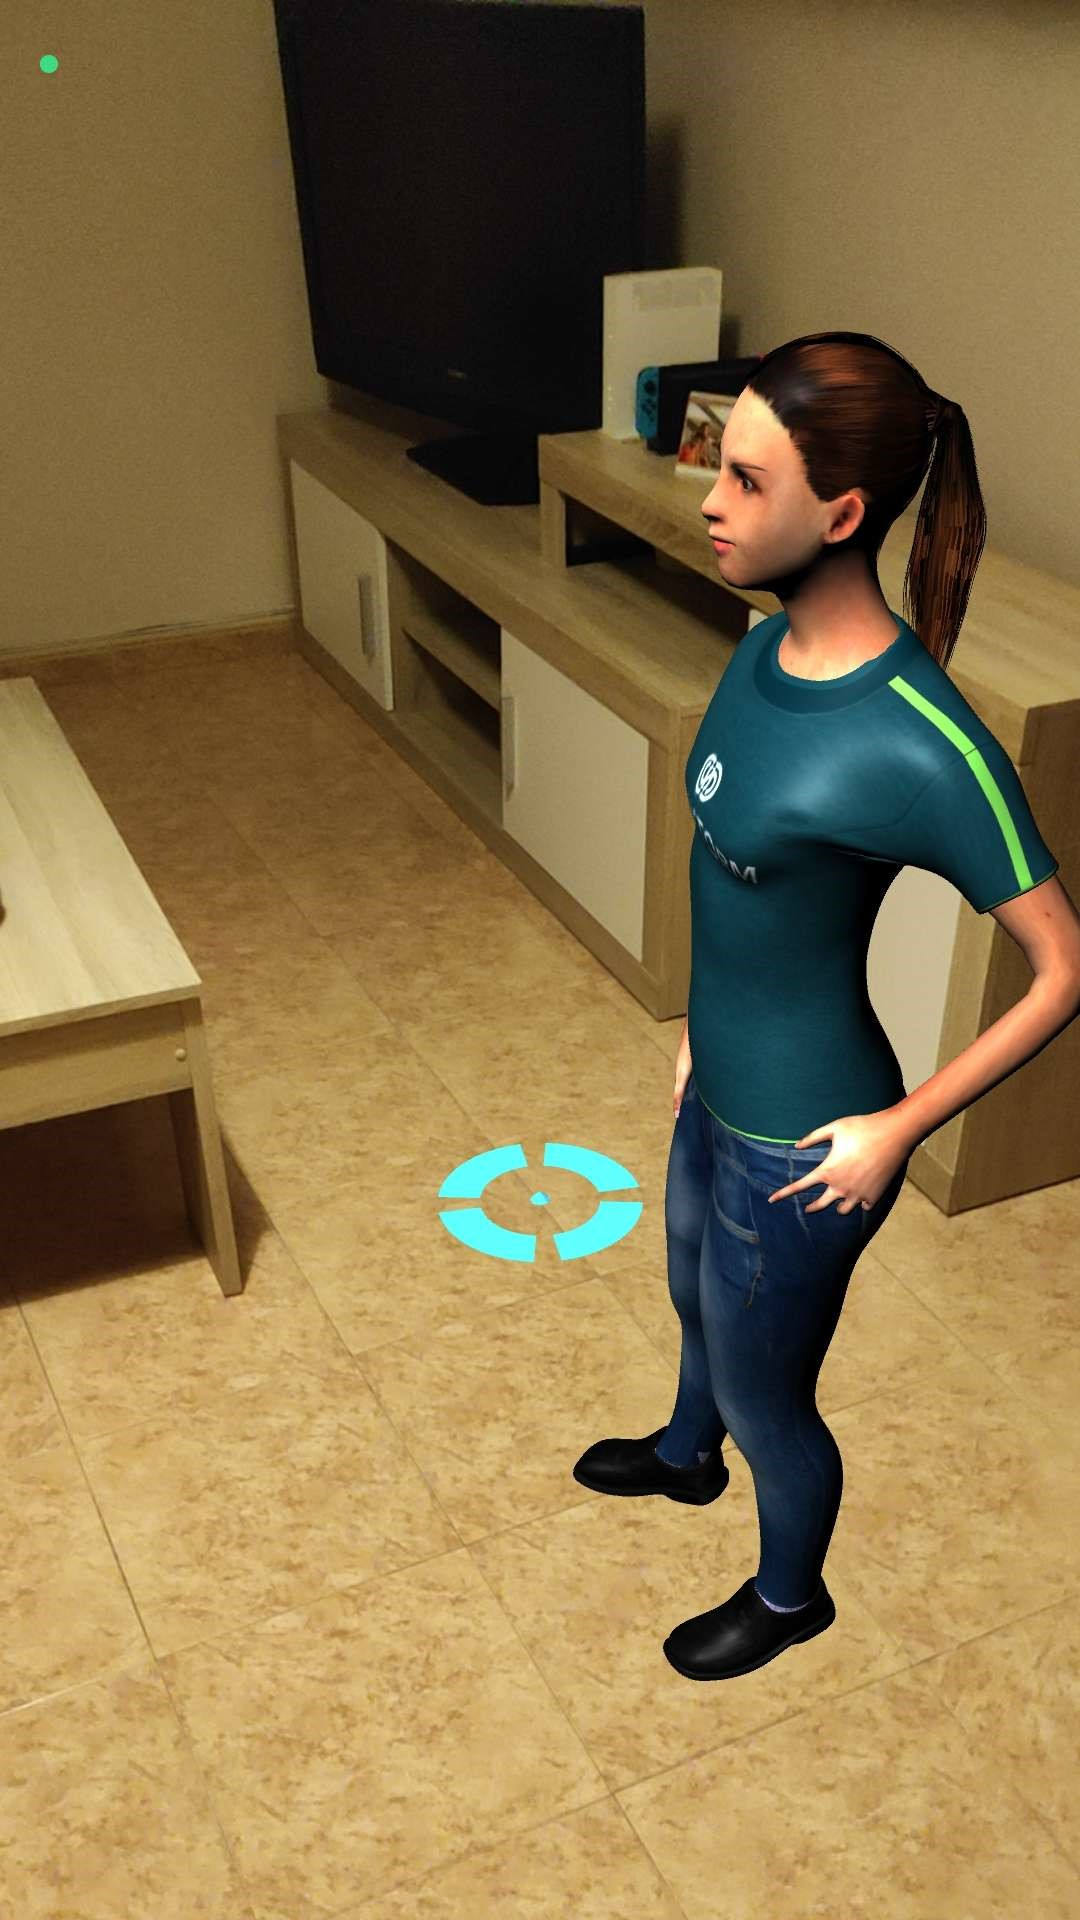
\includegraphics[width=0.2\textwidth]{7_end_of_animation.jpg}
\caption{La retícula vuelve a aparecer al terminar la animación.}
\label{fig:7_end_of_animation}
\end{figure}

        \paragraph{}
        Una vez termine la animación y el discurso volverá a aparecer la retícula, indicando al usuario que puede volver a pulsar sobre la pantalla para que vuelva a comenzar el discurso y la animación (figura \ref{fig:7_end_of_animation}. Para cerrar la sesión de \ra, el usuario podrá pulsar el botón de <<volver>> del móvil, con lo que, de manera previa, se finalizarán la animación y el audio.

\end{document}